\documentclass[12pt,a4paper]{article}
\usepackage{amsmath, amssymb}
\usepackage{geometry}
\usepackage{hyperref}
\usepackage{booktabs}
\usepackage{graphicx}
\usepackage{setspace}
\usepackage{float}
\usepackage{xcolor}
\usepackage{tikz}
\usetikzlibrary{positioning,arrows.meta,shapes.geometric}
\graphicspath{{assets/}}

%title page
\geometry{margin=1in}
\onehalfspacing

\begin{document}

% Title Page
\begin{titlepage}
    \centering
        
    \Huge
    \textbf{Jaypee Institute of Information Technology, Sector - 62, Noida } \\
    \vspace{0.5cm}
    \Large
    \textbf{B.Tech CSE III Semester}\\
    \vspace{1cm}
        
    \includegraphics[scale=0.2]{jiit_logo}\\
        
    \vspace{1cm}
    \Huge
    \textbf{DBMS Lab PBL Report}\\
    \Large
        
    \textbf{Ecommerce Database Explorer}\\
    \vspace{1cm}
    
    \Large
    \textbf{Submitted to}\\
    Dr. Indu Chawla\\
    Dr. Parmeet Kaur Sodhi\\
    Dr. Prateek Soni\\[0.5cm]
    
    \textbf{Submitted by}
    \vspace{0.5cm}
    
    \begin{tabular}{lll}
        Harsh Sharma      & 2401030232 & B5 \\
        Karvy Singh       & 2401030234 & B5 \\
        Rudra Kumar Singh & 2401030237 & B5 \\
    \end{tabular}
    
    \vspace*{\fill}
    \normalsize
\end{titlepage}

%letter of transmittal 
\begin{center}
    \Large\textbf{Letter of Transmittal}
\end{center}
\vspace{1cm}

\noindent
\textbf{Dr. Indu Chawla}\\
\textbf{Dr. Parmeet Kaur Sodhi}\\
\textbf{Dr. Prateek Soni}\\
[0.5em]
Department of Computer Science \& IT\\
[0.5em]

\vspace{1cm}

\noindent
\textbf{Subject:} Submission of Project ``Ecommerce Database Explorer''

\vspace{1cm}

\noindent
Respected Madam/Sir,

\vspace{1em}

\noindent
We are pleased to submit our project titled \textit{``Ecommerce Database Explorer''} as part of our DBMS laboratory course. This report documents the design and implementation of a relational database for a simplified e--commerce platform, along with a web--based interface for exploring tables, routines, and database artifacts.

\vspace{1em}

\noindent
We have endeavored to cover the complete database life cycle starting from requirement analysis and conceptual design to logical schema, normalization, integrity constraints, and implementation of stored procedures, functions, and triggers using MySQL's procedural extensions (PL/SQL--style constructs). The main focus of the work is on database design quality, normal forms, and the use of relational algebra concepts such as joins, union, intersection, difference, and division, which are demonstrated through various stored routines.

\vspace{1em}

\noindent
We would like to thank you for your guidance and for providing us the opportunity to apply the theoretical concepts of DBMS to a practical e--commerce scenario.

\vspace{1em}

\noindent
Sincerely, \\[1em]

\noindent
Harsh Sharma (2401030232)\\
Karvy Singh (2401030234)\\
Rudra Kumar Singh (2401030237)\\

\vspace{1cm}

\noindent
Date: \today

\newpage

\tableofcontents

\newpage

\section{Introduction}

Electronic commerce platforms are typical examples of data--intensive applications where database design plays a central role. They involve multiple interacting entities such as customers, sellers, products, orders, reviews, and pricing histories. The quality of the underlying relational schema directly affects correctness, performance, and extensibility of the overall system.

In this project, we designed and implemented an \textbf{Ecommerce Database Explorer} using \textbf{MySQL} as the relational database management system. On top of the database, we built a lightweight web interface using \textbf{FastAPI} and vanilla HTML/JavaScript to browse tables and to experiment with Data Definition Language (DDL), Data Manipulation Language (DML), and stored routines.

The primary emphasis of the project is on:
\begin{itemize}
    \item Systematic relational database design.
    \item Achieving higher normal forms and eliminating redundancy.
    \item Implementing business logic using PL/SQL--style stored procedures, functions and triggers.
    \item Demonstrating relational algebra concepts such as joins, union, intersection, difference, division, and aggregation using real stored routines.
\end{itemize}

The web API and front--end are intentionally kept simple and minimal, serving mainly as a convenient explorer for the underlying database design and its artifacts.

\section{Objectives}

The main objectives of the project are:
\begin{enumerate}
    \item To model a realistic yet manageable e--commerce domain using an Entity--Relationship (ER) approach.
    \item To transform the ER model into a normalized relational schema in MySQL, satisfying at least Third Normal Form (3NF) and, where possible, Boyce--Codd Normal Form (BCNF).
    \item To implement integrity constraints using primary keys, foreign keys, unique constraints and \texttt{CHECK} constraints.
    \item To encapsulate business logic using PL/SQL--style stored procedures, functions, and triggers.
    \item To demonstrate relational algebra operations (joins, union, intersection, difference, division) using stored routines.
    \item To provide a small web--based interface for exploring tables, modifying data, and invoking database routines.
\end{enumerate}

\section{System Overview}

At a high level, the system consists of:
\begin{itemize}
    \item A MySQL database named \texttt{dbms} containing all the tables, constraints, stored procedures, functions, and triggers.
    \item A FastAPI back--end (\texttt{app.py}) that connects to the MySQL database and exposes HTTP endpoints for:
    \begin{itemize}
        \item Listing tables and table contents.
        \item Describing table schemas.
        \item Creating, dropping, and truncating tables (DDL).
        \item Inserting, updating, and deleting rows (DML).
        \item Invoking stored procedures and functions.
    \end{itemize}
    \item A set of static HTML pages:
    \begin{itemize}
        \item \texttt{index.html}: Simple table viewer.
        \item \texttt{editor.html}: Interactive table editor supporting row update and delete.
        \item \texttt{ddl.html}: DDL explorer for creating, dropping, and truncating tables.
        \item \texttt{artifacts.html}: Routine explorer to invoke procedures and functions documented in the \texttt{DbArtifacts} table.
    \end{itemize}
\end{itemize}

The following sections focus primarily on the database design aspects: ER modeling, relational schema, normalization, relational algebra, and PL/SQL constructs.

\section{Requirements Analysis}

The simplified e--commerce system is designed to support the following core requirements:

\begin{itemize}
    \item \textbf{Manage users}: Two distinct types of users are supported: \emph{customers} and \emph{sellers}. Both have login credentials and contact details.
    \item \textbf{Manage products}: Sellers can list products for sale with name, price, stock quantity, description and rating.
    \item \textbf{Handle orders}: Customers can place orders for products in certain quantities. Stock is decremented accordingly.
    \item \textbf{Shopping cart}: Customers can maintain a cart with one or more items before placing orders.
    \item \textbf{Reviews}: Customers can rate and review products. Each customer can review a product at most once.
    \item \textbf{Price history}: Changes in product price should be logged for auditing.
    \item \textbf{Analytical queries}: The system should support queries such as total spend by a customer, total revenue of a seller, loyal customers who have bought all products of a seller, and aggregated order statistics.
\end{itemize}

From these requirements, we derived the main entities: \texttt{Customers}, \texttt{Sellers}, \texttt{Products}, \texttt{Orders}, \texttt{CartItems}, \texttt{Reviews}, \texttt{ProductPriceHistory}, and \texttt{DbArtifacts}.

\section{Conceptual Design: ER Diagram}

% Figure~\ref{fig:er} shows a ER diagram of the e--commerce database.

\begin{figure}[p]
\centering
\rotatebox{90}{%
  \resizebox{0.9\textheight}{!}{%
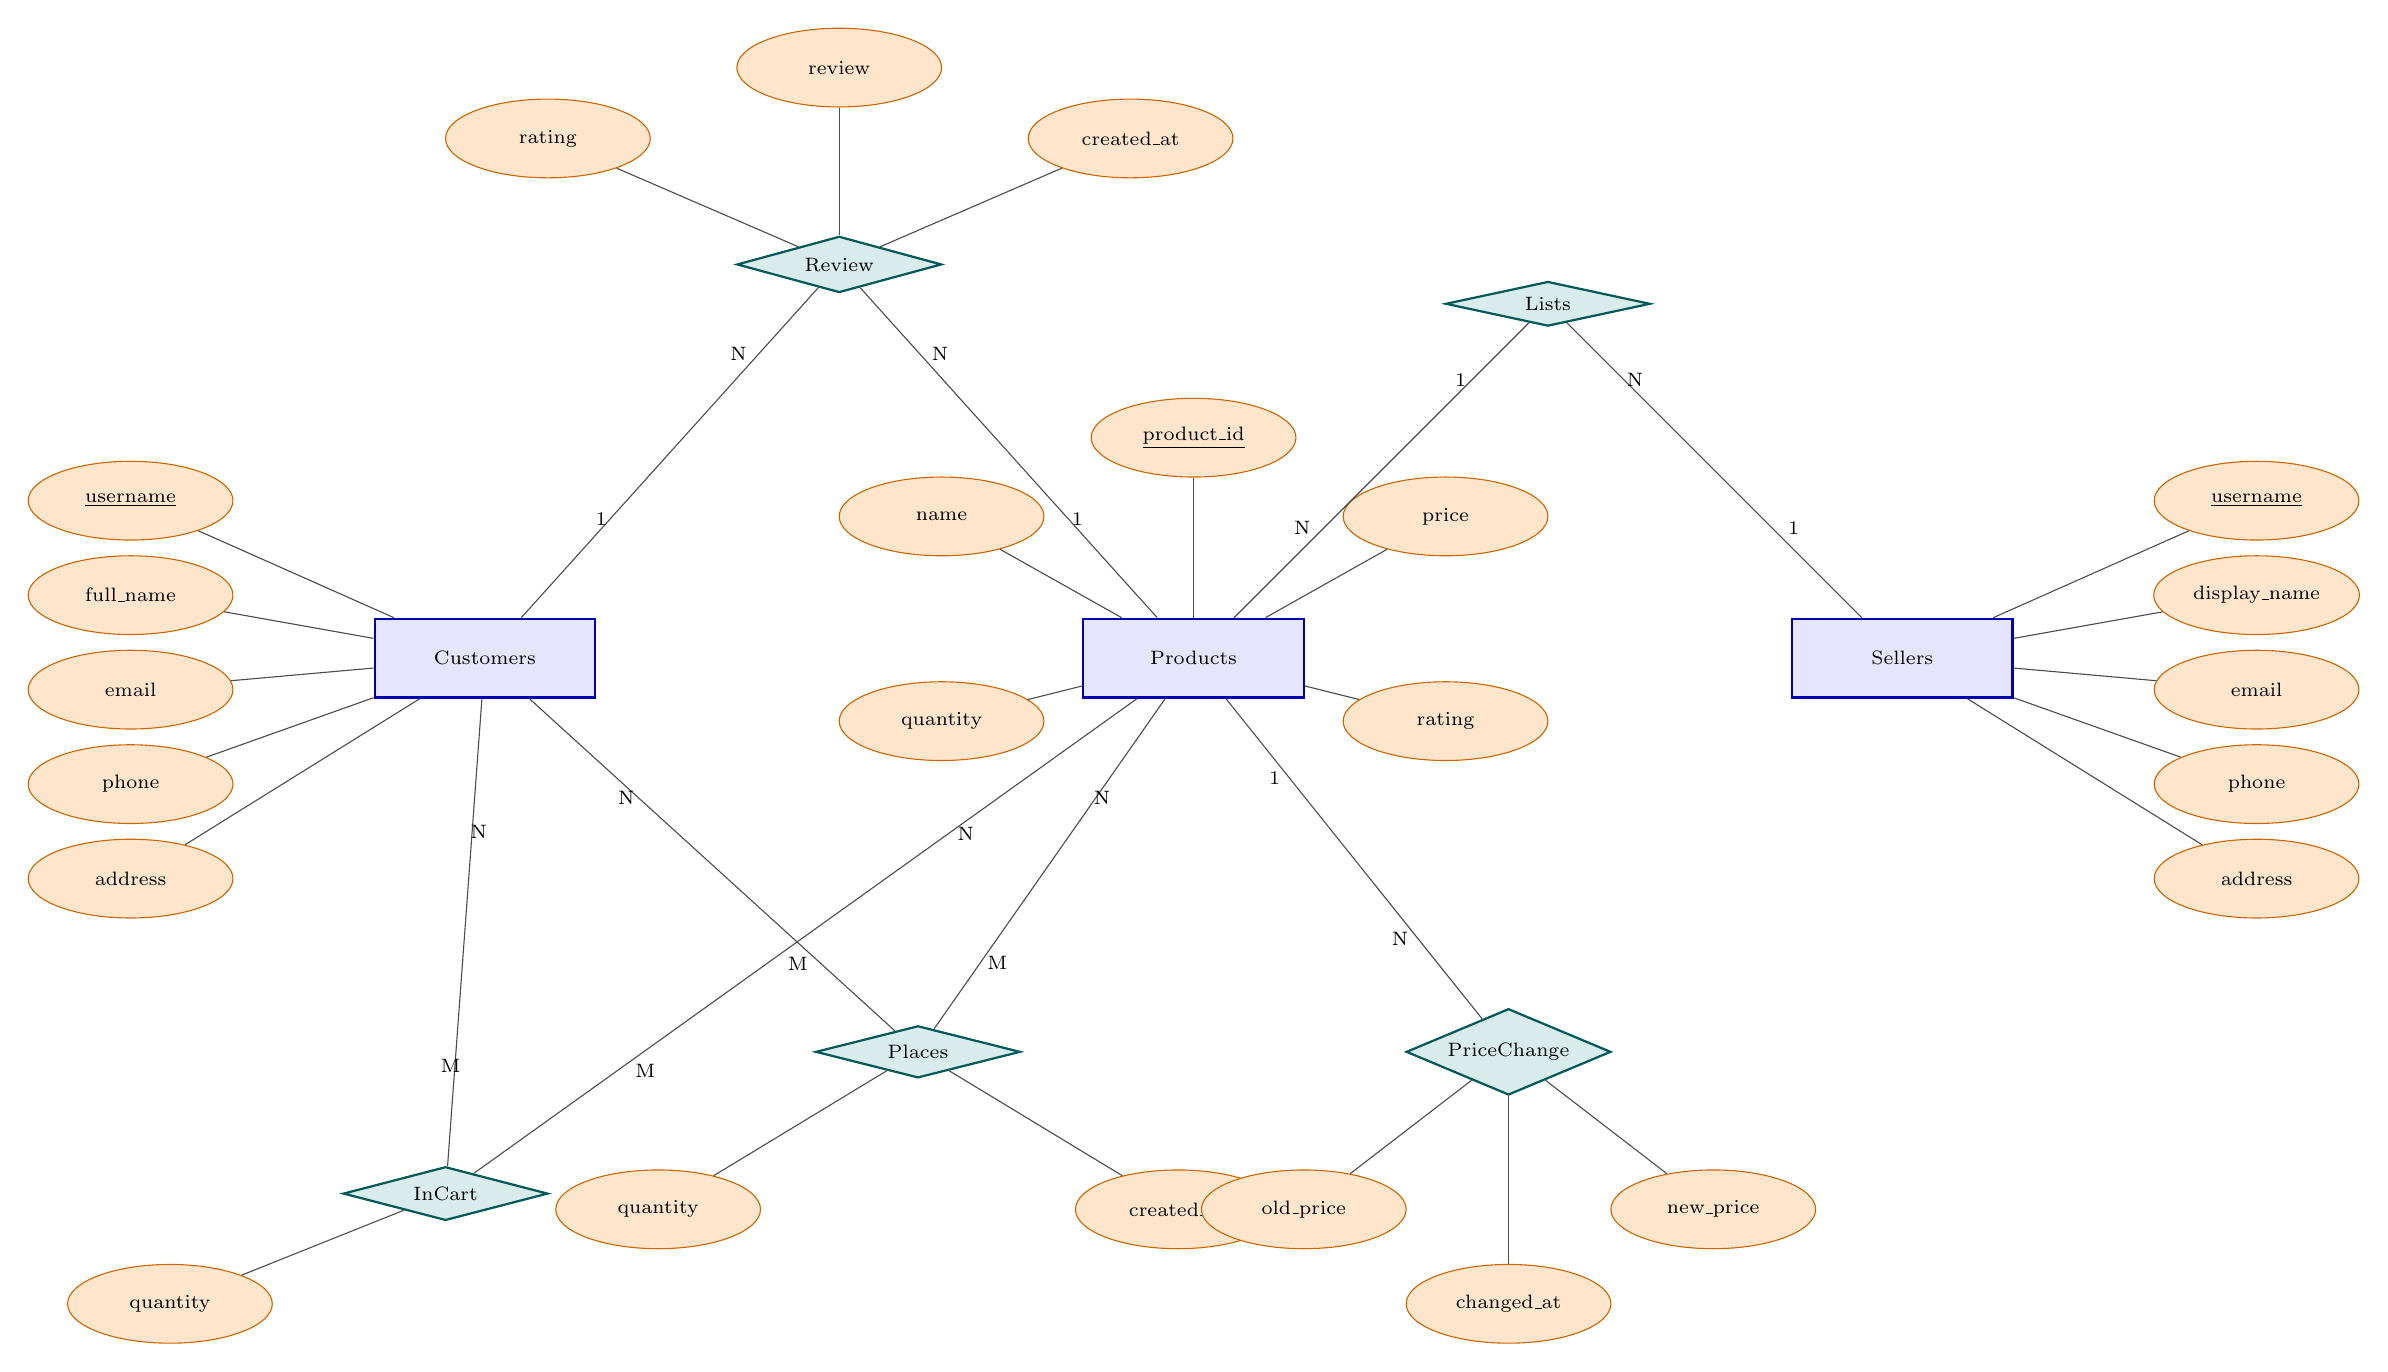
\begin{tikzpicture}[
    entity/.style={
      rectangle,
      draw=blue!70!black,
      fill=blue!10,
      thick,
      minimum width=2.8cm,
      minimum height=1cm
    },
    relationship/.style={
      diamond,
      draw=teal!70!black,
      fill=teal!15,
      thick,
      aspect=2,
      minimum width=2.6cm,
      inner sep=1pt
    },
    attribute/.style={
      ellipse,
      draw=orange!80!black,
      fill=orange!20,
      minimum width=2.6cm,
      minimum height=1cm
    },
    rel/.style={
      draw=black!70,
      >=Stealth
    },
    every node/.style={font=\scriptsize}
  ]

  %========================================
  % ENTITIES
  %========================================
  \node[entity] (Customer) at (-9, 0) {Customers};
  \node[entity] (Product)  at (  0, 0) {Products};
  \node[entity] (Seller)   at (  9, 0) {Sellers};

  %========================================
  % RELATIONSHIPS (DIAMONDS)
  %========================================
  % Customer–Product: Review
  \node[relationship] (RelReview) at (-4.5, 5) {Review};

  % Customer–Product: Order
  \node[relationship] (RelOrder)  at (-3.5, -5) {Places};

  % Customer–Product: Cart
  \node[relationship] (RelCart)   at (-9.5, -6.8) {InCart};

  % Seller–Product: Lists
  \node[relationship] (RelLists)  at ( 4.5, 4.5) {Lists};

  % Product: Price change
  \node[relationship] (RelPrice)  at ( 4.0, -5) {PriceChange};

  %========================================
  % CUSTOMER ATTRIBUTES
  %========================================
  \node[attribute] (C_username) at (-13.5,  2.0) {\underline{username}};
  \node[attribute] (C_fullname) at (-13.5,  0.8) {full\_name};
  \node[attribute] (C_email)    at (-13.5, -0.4) {email};
  \node[attribute] (C_phone)    at (-13.5, -1.6) {phone};
  \node[attribute] (C_address)  at (-13.5, -2.8) {address};

  \draw[rel] (Customer) -- (C_username);
  \draw[rel] (Customer) -- (C_fullname);
  \draw[rel] (Customer) -- (C_email);
  \draw[rel] (Customer) -- (C_phone);
  \draw[rel] (Customer) -- (C_address);

  %========================================
  % PRODUCT ATTRIBUTES
  %========================================
  \node[attribute] (P_id)      at (  0,  2.8) {\underline{product\_id}};
  \node[attribute] (P_name)    at ( -3.2, 1.8) {name};
  \node[attribute] (P_price)   at (  3.2, 1.8) {price};
  \node[attribute] (P_qty)     at ( -3.2,-0.8) {quantity};
  \node[attribute] (P_rating)  at (  3.2,-0.8) {rating};

  \draw[rel] (Product) -- (P_id);
  \draw[rel] (Product) -- (P_name);
  \draw[rel] (Product) -- (P_price);
  \draw[rel] (Product) -- (P_qty);
  \draw[rel] (Product) -- (P_rating);

  %========================================
  % SELLER ATTRIBUTES
  %========================================
  \node[attribute] (S_username) at ( 13.5,  2.0) {\underline{username}};
  \node[attribute] (S_display)  at ( 13.5,  0.8) {display\_name};
  \node[attribute] (S_email)    at ( 13.5, -0.4) {email};
  \node[attribute] (S_phone)    at ( 13.5, -1.6) {phone};
  \node[attribute] (S_address)  at ( 13.5, -2.8) {address};

  \draw[rel] (Seller) -- (S_username);
  \draw[rel] (Seller) -- (S_display);
  \draw[rel] (Seller) -- (S_email);
  \draw[rel] (Seller) -- (S_phone);
  \draw[rel] (Seller) -- (S_address);

  %========================================
  % REVIEW RELATIONSHIP ATTRIBUTES
  %========================================
  \node[attribute] (R_rating)  at (-8.2, 6.6) {rating};
  \node[attribute] (R_review)  at (-4.5, 7.5) {review};
  \node[attribute] (R_created) at (-0.8, 6.6) {created\_at};

  \draw[rel] (RelReview) -- (R_rating);
  \draw[rel] (RelReview) -- (R_review);
  \draw[rel] (RelReview) -- (R_created);

  %========================================
  % ORDER RELATIONSHIP ATTRIBUTES
  %========================================
  \node[attribute] (O_qty)     at (-6.8, -7.0) {quantity};
  \node[attribute] (O_created) at (-0.2, -7.0) {created\_at};

  \draw[rel] (RelOrder) -- (O_qty);
  \draw[rel] (RelOrder) -- (O_created);

  %========================================
  % CART RELATIONSHIP ATTRIBUTE
  %========================================
  \node[attribute] (Cart_qty) at (-13.0, -8.2) {quantity};
  \draw[rel] (RelCart) -- (Cart_qty);

  %========================================
  % PRICE CHANGE RELATIONSHIP ATTRIBUTES
  %========================================
  \node[attribute] (PH_old)     at ( 1.4, -7.0) {old\_price};
  \node[attribute] (PH_new)     at ( 6.6, -7.0) {new\_price};
  \node[attribute] (PH_changed) at ( 4.0, -8.2) {changed\_at};

  \draw[rel] (RelPrice) -- (PH_old);
  \draw[rel] (RelPrice) -- (PH_new);
  \draw[rel] (RelPrice) -- (PH_changed);

  %========================================
  % CONNECTIONS + CARDINALITIES
  %========================================

  % Customer -- Review (1 to N on both sides -> M:N)
  \draw[rel] (Customer) -- node[near start, above, xshift=2pt]{1}
                         node[near end,   above, xshift=-2pt]{N}
                         (RelReview);
  \draw[rel] (Product) -- node[near start, above, xshift=-2pt]{1}
                        node[near end,   above, xshift=2pt]{N}
                        (RelReview);

  % Customer -- Places (Orders) (M:N)
  \draw[rel] (Customer) -- node[near start, below, xshift=2pt]{N}
                          node[near end,   below, xshift=-2pt]{M}
                          (RelOrder);
  \draw[rel] (Product) -- node[near start, below, xshift=-2pt]{N}
                         node[near end,   below, xshift=2pt]{M}
                         (RelOrder);

  % Customer -- InCart (M:N)
  \draw[rel] (Customer) -- node[near start, below, xshift=2pt]{N}
                          node[near end,   below, xshift=-2pt]{M}
                          (RelCart);
  \draw[rel] (Product) -- node[near start, below, xshift=-2pt]{N}
                         node[near end,   below, xshift=2pt]{M}
                         (RelCart);

  % Seller -- Lists -- Product (1:N from Seller to Product)
  \draw[rel] (Seller) -- node[near start, above, xshift=2pt]{1}
                         node[near end,   above, xshift=-2pt]{N}
                         (RelLists);
  \draw[rel] (Product) -- node[near start, above, xshift=-2pt]{N}
                          node[near end,   above, xshift=2pt]{1}
                          (RelLists);

  % Product -- PriceChange (1:N)
  \draw[rel] (Product) -- node[near start, left]{1}
                          node[near end,   left]{N}
                          (RelPrice);

\end{tikzpicture}%
  }% end resizebox
}% end rotatebox
\caption{ER diagram for the Ecommerce Database Explorer}\\
\end{figure}

The main cardinalities are:
\begin{itemize}
    \item One customer can have many cart items and many orders.
    \item One seller can list many products.
    \item One product can have many reviews and many price history entries.
    \item Each review belongs to exactly one customer and one product.
    \item Each order entry is for exactly one customer and one product.
\end{itemize}

\section{Logical Design: Relational Schema}

The ER model is mapped to the following relational tables in MySQL:

\subsection{Core Entity Tables}

\subsubsection{Customers}

\begin{verbatim}
CREATE TABLE Customers (
  username       VARCHAR(64)  PRIMARY KEY,
  password_hash  VARCHAR(255) NOT NULL,
  full_name      VARCHAR(255) NOT NULL,
  email          VARCHAR(255) NOT NULL UNIQUE,
  phone          VARCHAR(32),
  address        TEXT,
  created_at     DATETIME NOT NULL DEFAULT CURRENT_TIMESTAMP
);
\end{verbatim}

\textbf{Key points:}
\begin{itemize}
    \item \texttt{username} is the primary key.
    \item \texttt{email} is unique, making it an alternate key.
    \item All attributes are atomic, satisfying 1NF.
\end{itemize}

\subsubsection{Sellers}

\begin{verbatim}
CREATE TABLE Sellers (
  username       VARCHAR(64)  PRIMARY KEY,
  password_hash  VARCHAR(255) NOT NULL,
  display_name   VARCHAR(255) NOT NULL,
  email          VARCHAR(255) NOT NULL UNIQUE,
  phone          VARCHAR(32),
  address        TEXT,
  created_at     DATETIME NOT NULL DEFAULT CURRENT_TIMESTAMP
);
\end{verbatim}

The design is analogous to \texttt{Customers}, keeping customer and seller data separate while enforcing similar constraints.

\subsubsection{Products}

\begin{verbatim}
CREATE TABLE Products (
  product_id       INT UNSIGNED NOT NULL AUTO_INCREMENT,
  seller_username  VARCHAR(64)  NOT NULL,
  name             VARCHAR(255) NOT NULL,
  rating           INT,
  price            INT UNSIGNED NOT NULL,
  quantity         INT UNSIGNED NOT NULL,
  description      TEXT,
  created_at       DATETIME NOT NULL DEFAULT CURRENT_TIMESTAMP,
  PRIMARY KEY (product_id),
  FOREIGN KEY (seller_username) REFERENCES Sellers(username)
    ON DELETE CASCADE,
  CHECK (price >= 0),
  CHECK (quantity >= 0),
  CHECK (rating IS NULL OR rating BETWEEN 1 AND 5),
  UNIQUE KEY uq_products_seller_name (seller_username, name)
);
\end{verbatim}

\textbf{Key points:}
\begin{itemize}
    \item \texttt{product_id} is the primary key.
    \item The pair \texttt{(seller\_username, name)} is unique, preventing a seller from listing two products with the same name.
    \item \texttt{CHECK} constraints enforce data validity for price, quantity, and rating.
\end{itemize}

\subsection{Relationship Tables}

\subsubsection{Reviews}

\begin{verbatim}
CREATE TABLE Reviews (
  product_id         INT UNSIGNED NOT NULL,
  customer_username  VARCHAR(64)  NOT NULL,
  rating             INT NOT NULL,
  review             TEXT,
  created_at         DATETIME NOT NULL DEFAULT CURRENT_TIMESTAMP,
  PRIMARY KEY (product_id, customer_username),
  FOREIGN KEY (product_id) REFERENCES Products(product_id)
    ON DELETE CASCADE,
  FOREIGN KEY (customer_username) REFERENCES Customers(username)
    ON DELETE CASCADE,
  CHECK (rating BETWEEN 1 AND 5)
);
\end{verbatim}

Each customer can review a product at most once, which is enforced by the composite primary key.

\subsubsection{CartItems}

\begin{verbatim}
CREATE TABLE CartItems (
  product_id         INT UNSIGNED NOT NULL,
  customer_username  VARCHAR(64)  NOT NULL,
  quantity           INT UNSIGNED NOT NULL,
  PRIMARY KEY (product_id, customer_username),
  FOREIGN KEY (product_id) REFERENCES Products(product_id)
    ON DELETE CASCADE,
  FOREIGN KEY (customer_username) REFERENCES Customers(username)
    ON DELETE CASCADE,
  CHECK (quantity >= 0)
);
\end{verbatim}

\subsubsection{Orders}

\begin{verbatim}
CREATE TABLE Orders (
  product_id         INT UNSIGNED NOT NULL,
  customer_username  VARCHAR(64)  NOT NULL,
  quantity           INT UNSIGNED NOT NULL,
  created_at         DATETIME NOT NULL DEFAULT CURRENT_TIMESTAMP,
  PRIMARY KEY (product_id, customer_username, created_at),
  FOREIGN KEY (product_id) REFERENCES Products(product_id)
    ON DELETE RESTRICT,
  FOREIGN KEY (customer_username) REFERENCES Customers(username)
    ON DELETE RESTRICT,
  CHECK (quantity >= 0)
);
\end{verbatim}

The primary key includes \texttt{created\_at} so that the same customer can place multiple orders for the same product at different times.

\subsection{Supporting Tables}

\subsubsection{ProductPriceHistory}

\begin{verbatim}
CREATE TABLE ProductPriceHistory (
  id         INT UNSIGNED NOT NULL AUTO_INCREMENT,
  product_id INT UNSIGNED NOT NULL,
  old_price  INT UNSIGNED NOT NULL,
  new_price  INT UNSIGNED NOT NULL,
  changed_at DATETIME NOT NULL DEFAULT CURRENT_TIMESTAMP,
  PRIMARY KEY (id),
  FOREIGN KEY (product_id) REFERENCES Products(product_id)
    ON DELETE CASCADE
);
\end{verbatim}

This table records every price change for a product, populated via a trigger (see Section~\ref{sec:triggers}).

\subsubsection{DbArtifacts}

\begin{verbatim}
CREATE TABLE DbArtifacts (
  name         VARCHAR(128) NOT NULL,
  type         VARCHAR(16)  NOT NULL,
  description  TEXT         NOT NULL,
  param_count  INT          NOT NULL DEFAULT 0,
  PRIMARY KEY (name, type),
  CHECK (type IN ('PROCEDURE','FUNCTION','TRIGGER')),
  CHECK (param_count >= 0)
);
\end{verbatim}

This is a documentation table that stores metadata about procedures, functions, and triggers. The \texttt{artifacts.html} page reads from this table to dynamically present available routines and their parameter counts.

\section{Normalization and Normal Forms}

All tables were designed to satisfy at least Third Normal Form (3NF). In many cases the schema also satisfies Boyce--Codd Normal Form (BCNF).

\subsection{Customers and Sellers}

\textbf{Functional dependencies} in \texttt{Customers}:
\[
\text{username} \rightarrow \{\text{password\_hash}, \text{full\_name}, \text{email}, \text{phone}, \text{address}, \text{created\_at}\}
\]
\[
\text{email} \rightarrow \{\text{username}, \text{password\_hash}, \text{full\_name}, \text{phone}, \text{address}, \text{created\_at}\}
\]

Both \texttt{username} and \texttt{email} are candidate keys. All non--key attributes depend on the whole key and only on the key.

\begin{itemize}
    \item 1NF: All attributes are atomic (no repeating groups).
    \item 2NF: There is no composite key, so 2NF is trivially satisfied.
    \item 3NF: No non--key attribute depends on another non--key attribute; hence 3NF holds.
    \item BCNF: Every non--trivial functional dependency has a candidate key on the left; therefore \texttt{Customers} and \texttt{Sellers} are in BCNF.
\end{itemize}

\subsection{Products}

Main functional dependencies in \texttt{Products}:
\[
\text{product\_id} \rightarrow \{\text{seller\_username}, \text{name}, \text{rating}, \text{price}, \text{quantity}, \text{description}, \text{created\_at}\}
\]
\[
(\text{seller\_username},\text{name}) \rightarrow \{\text{product\_id}, \text{rating}, \text{price}, \text{quantity}, \text{description}, \text{created\_at}\}
\]

Both \texttt{product\_id} and the pair \texttt{(seller\_username, name)} are candidate keys due to the unique constraint.

There are no partial or transitive dependencies among non--key attributes. Thus:
\begin{itemize}
    \item \texttt{Products} is in 3NF.
    \item All determining attributes on the left side of FDs are candidate keys, so it also satisfies BCNF.
\end{itemize}

\subsection{Relationship Tables: Reviews, CartItems, Orders}

\texttt{Reviews} has primary key \texttt{(product\_id, customer\_username)} and other attributes \texttt{rating, review, created\_at}. The only relevant FD is:
\[
(\text{product\_id},\ \text{customer\_username}) \rightarrow \{\text{rating}, \text{review}, \text{created\_at}\}
\]

Similar reasoning applies to \texttt{CartItems} and \texttt{Orders}.

\begin{itemize}
    \item All attributes are atomic: 1NF.
    \item All non--key attributes depend on the full composite key: 2NF.
    \item There are no transitive dependencies: 3NF.
    \item Left side of each FD is a key: hence BCNF.
\end{itemize}

\subsection{Supporting Tables}

\texttt{ProductPriceHistory} and \texttt{DbArtifacts} are also in at least 3NF:
\begin{itemize}
    \item Each table has a simple primary key (\texttt{id} for \texttt{ProductPriceHistory}, and \texttt{(name, type)} for \texttt{DbArtifacts}).
    \item All other attributes depend solely on that key.
    \item No non--key attribute determines any other non--key attribute.
\end{itemize}

Thus the overall schema is free of update, insertion, and deletion anomalies related to redundancy.

\section{Integrity Constraints and Business Rules}

Beyond primary and foreign keys, the database enforces various integrity rules:

\begin{itemize}
    \item \textbf{Domain constraints}: \texttt{CHECK} constraints ensure non--negative prices and quantities and enforce valid rating ranges.
    \item \textbf{Referential integrity}: Foreign keys connect \texttt{Orders}, \texttt{CartItems}, and \texttt{Reviews} to \texttt{Products}, \texttt{Customers}, and \texttt{Sellers} with appropriate \texttt{ON DELETE} actions.
    \item \textbf{Uniqueness constraints}: Unique keys on \texttt{email} and on \texttt{(seller\_username, name)} avoid duplicates.
    \item \textbf{Triggers}: Before/after triggers check business rules such as stock availability, rating range, non--zero cart quantities, and automatic stock decrement and rating updates.
\end{itemize}

\section{PL/SQL Layer: Procedures, Functions and Triggers}
\label{sec:triggers}

MySQL procedural SQL (PL/SQL--style syntax) is used to encapsulate business logic inside the database.

\subsection{Stored Procedures}

\subsubsection{\texttt{create\_customer} and \texttt{create\_seller}}

These procedures insert new rows into \texttt{Customers} and \texttt{Sellers} respectively:

\begin{verbatim}
CREATE PROCEDURE create_customer(
  IN p_username      VARCHAR(64),
  IN p_password_hash VARCHAR(255),
  IN p_full_name     VARCHAR(255),
  IN p_email         VARCHAR(255),
  IN p_phone         VARCHAR(32),
  IN p_address       TEXT
)
BEGIN
  INSERT INTO Customers(username, password_hash, full_name,
                        email, phone, address)
  VALUES (p_username, p_password_hash, p_full_name,
          p_email, p_phone, p_address);
END;
\end{verbatim}

These procedures support controlled creation of users, centralizing validation and allowing reuse.

\subsubsection{\texttt{add\_product}}

\begin{verbatim}
CREATE PROCEDURE add_product(
  IN p_seller_username VARCHAR(64),
  IN p_name            VARCHAR(255),
  IN p_price           INT UNSIGNED,
  IN p_quantity        INT UNSIGNED,
  IN p_description     TEXT
)
BEGIN
  INSERT INTO Products(seller_username, name, rating,
                       price, quantity, description)
  VALUES (p_seller_username, p_name, NULL,
          p_price, p_quantity, p_description);
END;
\end{verbatim}

\subsubsection{\texttt{place\_order} with Transactional Logic}

\begin{verbatim}
CREATE PROCEDURE place_order(
  IN p_customer_username VARCHAR(64),
  IN p_product_id        INT UNSIGNED,
  IN p_quantity          INT UNSIGNED
)
BEGIN
  DECLARE v_stock INT;

  SELECT quantity INTO v_stock
  FROM Products
  WHERE product_id = p_product_id
  FOR UPDATE;

  IF v_stock IS NULL THEN
    SIGNAL SQLSTATE '45000'
      SET MESSAGE_TEXT = 'Product not found';
  ELSEIF v_stock < p_quantity THEN
    SIGNAL SQLSTATE '45000'
      SET MESSAGE_TEXT = 'Insufficient stock';
  ELSE
    INSERT INTO Orders(product_id, customer_username, quantity)
    VALUES (p_product_id, p_customer_username, p_quantity);

    UPDATE Products
    SET quantity = quantity - p_quantity
    WHERE product_id = p_product_id;
  END IF;
END;
\end{verbatim}

The \texttt{FOR UPDATE} clause locks the product row to prevent race conditions while checking and updating stock.

\subsubsection{\texttt{get\_invoice}: Example with UNION ALL}

\begin{verbatim}
CREATE PROCEDURE get_invoice(IN p_user VARCHAR(10))
BEGIN
  SELECT p.name AS product, o.quantity AS quantity,
         p.price * o.quantity AS price
  FROM Products p, Orders o
  WHERE o.customer_username = p_user
    AND o.product_id = p.product_id
  UNION ALL
  SELECT 'TOTAL' AS product,
         SUM(o.quantity) AS quantity,
         SUM(p.price * o.quantity) AS price
  FROM Products p, Orders o
  WHERE o.customer_username = p_user
    AND o.product_id = p.product_id;
END;
\end{verbatim}

The invoice procedure demonstrates a combination of join and aggregation plus union of detail rows with a total row.

\subsection{Stored Functions}

Several functions compute derived values:

\begin{itemize}
    \item \texttt{product\_avg\_rating(product\_id)}: Returns average rating for a product.
    \item \texttt{customer\_total\_spent(customer\_username)}: Total amount spent by a customer.
    \item \texttt{customer\_order\_count(customer\_username)}: Number of orders placed by a customer.
    \item \texttt{product\_stock(product\_id)}: Current stock quantity.
    \item \texttt{seller\_total\_revenue(seller\_username)}: Total revenue for a seller.
\end{itemize}

Example:

\begin{verbatim}
CREATE FUNCTION customer_total_spent(
  p_customer_username VARCHAR(64)
)
RETURNS INT
READS SQL DATA
BEGIN
  DECLARE v_total INT;
  SELECT IFNULL(SUM(o.quantity * p.price),0) INTO v_total
  FROM Orders o
  JOIN Products p ON p.product_id = o.product_id
  WHERE o.customer_username = p_customer_username;
  RETURN v_total;
END;
\end{verbatim}

This function corresponds to a relational algebra expression applying a join and aggregation (see Section~\ref{sec:relalg}).

\subsection{Triggers}

\subsubsection{Validation Triggers}

\begin{itemize}
    \item \texttt{reviews\_before\_insert\_rating} ensures rating is between 1 and 5.
\begin{verbatim}
CREATE TRIGGER reviews_before_insert_rating
BEFORE INSERT ON Reviews
FOR EACH ROW
BEGIN
  IF NEW.rating < 1 OR NEW.rating > 5 THEN
    SIGNAL SQLSTATE '45000'
      SET MESSAGE_TEXT = 'Rating must be between 1 and 5';
  END IF;
END;
\end{verbatim}

    \item \texttt{cartitems\_before\_insert\_quantity} enforces strictly positive cart quantities.
\end{itemize}

\subsubsection{Stock Management Triggers}

\begin{itemize}
    \item \texttt{orders\_before\_insert\_stock} checks stock before inserting an order.
    \item \texttt{orders\_after\_insert\_decrement\_stock} decrements product stock after each order.
\end{itemize}

These triggers cooperate with the \texttt{place\_order} procedure to ensure that stock never goes negative and that each order corresponds to available inventory.

\subsubsection{Price History Trigger}

\begin{verbatim}
CREATE TRIGGER products_after_update_price
AFTER UPDATE ON Products
FOR EACH ROW
BEGIN
  IF NEW.price <> OLD.price THEN
    INSERT INTO ProductPriceHistory(product_id, old_price, new_price)
    VALUES (NEW.product_id, OLD.price, NEW.price);
  END IF;
END;
\end{verbatim}

This automatically logs every price change in \texttt{ProductPriceHistory}.

\subsubsection{Rating Aggregation Trigger}

\begin{verbatim}
CREATE TRIGGER reviews_after_insert_update_product_rating
AFTER INSERT ON Reviews
FOR EACH ROW
BEGIN
  UPDATE Products p
  SET p.rating = (
    SELECT ROUND(AVG(r.rating))
    FROM Reviews r
    WHERE r.product_id = NEW.product_id
  )
  WHERE p.product_id = NEW.product_id;
END;
\end{verbatim}

The product's \texttt{rating} column is maintained as the rounded average of all review ratings for that product.

\section{Relational Algebra and Joins}
\label{sec:relalg}

Several procedures are designed specifically to demonstrate relational algebra operations using SQL.

\subsection{Join Operations}

\subsubsection{Inner Join: \texttt{join\_orders\_products\_inner}}

\begin{verbatim}
CREATE PROCEDURE join_orders_products_inner(
  IN p_customer_username VARCHAR(64)
)
BEGIN
  SELECT o.product_id, p.name, o.quantity,
         p.price * o.quantity AS total_price
  FROM Orders o
  JOIN Products p ON p.product_id = o.product_id
  WHERE o.customer_username = p_customer_username;
END;
\end{verbatim}

In relational algebra, this corresponds to:
\[
\pi_{\text{product\_id},\ \text{name},\ \text{quantity},\ \text{total\_price}}
\left(
  \sigma_{\text{customer\_username} = c}
  (\text{Orders})
  \;\Join_{\text{Orders.product\_id} = \text{Products.product\_id}}\;
  \text{Products}
\right)
\]

\subsubsection{Left Join: \texttt{join\_products\_reviews\_left}}

\begin{verbatim}
CREATE PROCEDURE join_products_reviews_left()
BEGIN
  SELECT p.product_id, p.name, r.customer_username, r.rating
  FROM Products p
  LEFT JOIN Reviews r ON r.product_id = p.product_id;
END;
\end{verbatim}

This shows all products, including those with no reviews (outer join).

\subsubsection{Right Join: \texttt{join\_sellers\_products\_right}}

\begin{verbatim}
CREATE PROCEDURE join_sellers_products_right()
BEGIN
  SELECT s.username AS seller_username,
         s.display_name, p.product_id, p.name
  FROM Products p
  RIGHT JOIN Sellers s ON p.seller_username = s.username;
END;
\end{verbatim}

Each seller appears even if they have no products, illustrating a right outer join.

\subsubsection{Full Join via UNION: \texttt{join\_products\_reviews\_full}}

\begin{verbatim}
CREATE PROCEDURE join_products_reviews_full()
BEGIN
  SELECT p.product_id, p.name, r.customer_username, r.rating
  FROM Products p
  LEFT JOIN Reviews r ON r.product_id = p.product_id
  UNION
  SELECT p.product_id, p.name, r.customer_username, r.rating
  FROM Products p
  RIGHT JOIN Reviews r ON r.product_id = p.product_id;
END;
\end{verbatim}

Since MySQL does not have a native full outer join, this procedure simulates it using a union of left and right joins.

\subsubsection{Cross Join: \texttt{join\_customers\_sellers\_cross}}

\begin{verbatim}
CREATE PROCEDURE join_customers_sellers_cross(
  IN p_limit INT
)
BEGIN
  SELECT c.username AS customer_username,
         s.username AS seller_username
  FROM Customers c
  CROSS JOIN Sellers s
  LIMIT p_limit;
END;
\end{verbatim}

This corresponds to the Cartesian product of \texttt{Customers} and \texttt{Sellers}, limited to a subset of pairs.

\subsection{Set Operations: Union, Intersection, Difference}

\subsubsection{Union: \texttt{ra\_union\_customers\_orders\_reviews}}

\begin{verbatim}
CREATE PROCEDURE ra_union_customers_orders_reviews()
BEGIN
  SELECT DISTINCT customer_username
  FROM Orders
  UNION
  SELECT DISTINCT customer_username
  FROM Reviews;
END;
\end{verbatim}

Relational algebra:
\[
\pi_{\text{customer\_username}}(\text{Orders}) \;\cup\;
\pi_{\text{customer\_username}}(\text{Reviews})
\]

\subsubsection{Intersection: \texttt{ra\_intersection\_customers\_orders\_reviews}}

\begin{verbatim}
CREATE PROCEDURE ra_intersection_customers_orders_reviews()
BEGIN
  SELECT DISTINCT o.customer_username
  FROM Orders o
  JOIN Reviews r
    ON r.customer_username = o.customer_username;
END;
\end{verbatim}

Relational algebra:
\[
\pi_{\text{customer\_username}}(\text{Orders}) \;\cap\;
\pi_{\text{customer\_username}}(\text{Reviews})
\]

\subsubsection{Difference: \texttt{ra\_difference\_customers\_orders\_not\_reviews}}

\begin{verbatim}
CREATE PROCEDURE ra_difference_customers_orders_not_reviews()
BEGIN
  SELECT DISTINCT o.customer_username
  FROM Orders o
  LEFT JOIN Reviews r
    ON r.customer_username = o.customer_username
  WHERE r.customer_username IS NULL;
END;
\end{verbatim}

Relational algebra:
\[
\pi_{\text{customer\_username}}(\text{Orders})
\;-\;
\pi_{\text{customer\_username}}(\text{Reviews})
\]

\subsection{Division: Loyal Customers}

\subsubsection{Relational Division: \texttt{ra\_division\_loyal\_customers}}

\begin{verbatim}
CREATE PROCEDURE ra_division_loyal_customers(
  IN p_seller_username VARCHAR(64)
)
BEGIN
  SELECT c.username
  FROM Customers c
  WHERE NOT EXISTS (
    SELECT 1
    FROM Products p
    WHERE p.seller_username = p_seller_username
      AND NOT EXISTS (
        SELECT 1
        FROM Orders o
        WHERE o.customer_username = c.username
          AND o.product_id = p.product_id
      )
  );
END;
\end{verbatim}

This procedure finds customers who have bought \emph{all} products from a given seller. In relational algebra terms, it corresponds to division:
\[
\pi_{\text{customer}}(O) \div \pi_{\text{product}}(P_s)
\]
where $O$ is the relation of customer--product orders and $P_s$ is the set of products of seller $s$.

\subsection{Aggregation: Grouping and Aggregate Functions}

\subsubsection{Aggregated Orders: \texttt{agg\_orders\_by\_customer}}

\begin{verbatim}
CREATE PROCEDURE agg_orders_by_customer(
  IN p_customer_username VARCHAR(64)
)
BEGIN
  SELECT
    p_customer_username AS customer_username,
    COUNT(*)                       AS order_count,
    SUM(o.quantity * p.price)      AS total_amount,
    AVG(o.quantity * p.price)      AS avg_order_value,
    MIN(o.quantity * p.price)      AS min_order_value,
    MAX(o.quantity * p.price)      AS max_order_value
  FROM Orders o
  JOIN Products p ON p.product_id = o.product_id
  WHERE o.customer_username = p_customer_username;
END;
\end{verbatim}

This uses \texttt{COUNT}, \texttt{SUM}, \texttt{AVG}, \texttt{MIN}, and \texttt{MAX}, which map directly to relational algebra's aggregation operator $\gamma$.

\section{Database Explorer Front--End (Brief Description)}

Although the project centers on the database, a minimal web interface has been implemented for convenience:

\begin{itemize}
    \item \textbf{Table viewer} (\texttt{index.html}): Allows users to select any table and display its contents as an HTML table.
    \item \textbf{Table editor} (\texttt{editor.html}): Provides interactive editing of table rows. Primary key columns are detected via \texttt{DESC} and used for \texttt{UPDATE} and \texttt{DELETE} operations through \texttt{/api/update\_table} and \texttt{/api/delete\_table}.
    \item \textbf{DDL explorer} (\texttt{ddl.html}): Enables creation of new tables with chosen columns and types, and supports dropping and truncating existing tables.
    \item \textbf{Routine explorer} (\texttt{artifacts.html}): Reads procedure/function metadata from \texttt{DbArtifacts} and dynamically renders input fields for parameters, allowing easy experimentation with stored routines demonstrating relational algebra and PL/SQL.
\end{itemize}

The front--end is intentionally simple and generic so that the design and behavior of the database layer remain the main focus.

\section{Testing and Sample Scenarios}

To validate the design and implementation, the following test scenarios were considered:

\begin{itemize}
    \item \textbf{User creation}: Creating customers and sellers using \texttt{create\_customer} and \texttt{create\_seller}, ensuring uniqueness of usernames and emails.
    \item \textbf{Product listing}: Adding products via \texttt{add\_product} and verifying foreign key relationships and check constraints.
    \item \textbf{Order placement}: Calling \texttt{place\_order} under different stock conditions:
    \begin{itemize}
        \item Sufficient stock: Order inserted and product quantity decremented.
        \item Insufficient stock: Error raised by trigger or procedure.
        \item Non--existent product: \texttt{SIGNAL} raised.
    \end{itemize}
    \item \textbf{Review insertion}: Attempting to insert valid and invalid ratings to test the rating validation trigger.
    \item \textbf{Price update}: Updating product price and verifying that entries are created in \texttt{ProductPriceHistory}.
    \item \textbf{Relational algebra routines}: Executing join and set operation procedures via \texttt{artifacts.html} and checking correctness of results (union, intersection, difference, division and aggregations).
\end{itemize}

\section{Conclusion}

The \textbf{Ecommerce Database Explorer} project demonstrates how theoretical concepts of relational database design can be applied to a realistic application domain. Starting from requirements, we constructed an ER model and a normalized relational schema in MySQL, enforced various integrity constraints, and implemented business rules and analytical queries using PL/SQL--style stored procedures, functions, and triggers.

The project also illustrates how core relational algebra operations---joins, union, intersection, difference, division, and aggregation---can be expressed and executed through stored routines. The minimal web interface built with FastAPI and HTML/JavaScript acts as a convenient front--end to explore and interact with the database.

Overall, the project helped us to:
\begin{itemize}
    \item Practically apply normal forms and evaluate the quality of a schema.
    \item Use MySQL's procedural capabilities to keep business logic close to the data.
    \item Bridge the gap between relational algebra theory and SQL implementations.
\end{itemize}

\section{Future Enhancements}

Possible improvements and extensions include:
\begin{itemize}
    \item Introducing a dedicated \texttt{Orders} header table with an \texttt{order\_id} and a separate \texttt{OrderItems} table.
    \item Adding more complex constraints, such as preventing multiple reviews by the same customer for the same product at the application level.
    \item Implementing indexing strategies and query optimization for large data volumes.
    \item Extending the web explorer with authentication and role--based access (customer vs. seller).
    \item Adding reporting dashboards using stored views and additional aggregation routines.
\end{itemize}

\bibliographystyle{plain}
\begin{thebibliography}{9}

\bibitem{elmasri}
R.~Elmasri and S.~Navathe.
\newblock \emph{Fundamentals of Database Systems}.
\newblock Pearson.

\bibitem{mysql}
MySQL 8.0 Reference Manual,
\newblock \url{https://dev.mysql.com/doc/}.

\end{thebibliography}

\end{document}
